\Chapter{Szoftveres technológiák}
A következő fejezetben a szoftveres, illetve a gyakorlati függőségekről fogok írni. Ezeket a technológiákat találtam a legjobbnak, szem előtt tartva az egyszerűséget, az ingyenes hozzáférést, illetve a sokoldalú felhasználhatóságot. A felsorolásban leginkább webes technológiák szerepelnek, hiszen így könnyebben lehet több platformra is elérhetővé tenni a programot.


\Section{HTML}

A HTML, avagy a HyperText Markup Language a W3C (World Wide Web Consortium) által támogatott, szabványosított leíró nyelv. Weboldalak szerkezeti leírására fejlesztették ki az 1993-as években, azóta több verzió is megjelent belőle, melyekben bővítették a készleteit. A HTML nyelv segítségével lehet elkészíteni a weboldalak vázát, melyet tovább szerkeszthetünk funkciók hozzáadásával, megjelenés beállításával. Egy HTML oldal három fő részből áll, HTML, HEAD és BODY részből.

\begin{HTML5}
<!DOCTYPE HTML>
<html lang="hu">
    <head>
        <meta charset="UTF-8">
        <title>Oldal cime</title>
        <link rel="stylesheet" href="css/style.css">
    </head>
    <body>
        <h2>Ez egy pelda oldal</h2>
        <p>Ez egy bekezdes</p>
        <script src="js/script.js"></script>
    </body>
</html>
\end{HTML5}

\noindent A szöveges fájl egy típusdefinícióval kezdődik, mely információ a böngészőnek szól, hogy tudja milyen formátumú. Ezután következhet a fejléc rész, mely a \codeword{<head>} tagek között található. Itt rögzíthetünk olyan paramétereket, amelyeket a böngésző nem fog megjeleníteni, például a szerző, a weboldal címe, vagy éppen a stílusleíró fálj elérési útvonala. Majd végül a törzs része jön az oldalnak, ami a \codeword{<body>} tagek között szerepel. Ez már a megjelenítendő részt tartalmazza, viszont például \codeword{<script>} tag is szerepelhet benne, ami nem feltétlen jelenít meg tartalmat, viszont a weboldallal együtt töltődik be, nem pedig előtte, ami jobb élményt nyújthat a felhasználóknak.

\Section{JavaScript}

A JavaScript egy programozási nyelv, melyet nagyon sok fontos alkalmazásban használnak manapság, elsősorban weboldalak fejlesztésére, de megjelenik a JavaScript a mobilalkalmazás fejlesztésben is. A JavaScript egy multiparadigmájú nyelv, mely támogatja az imperatív, deklaratív és objektumorientált stílusokat is, szintaxisát tekintve a Java nyelvhez hasonlítható. Osztályok helyett prototípusokat alkalmaz, ezzel megvalósítva az objektumorientált programozást. A JavaScript továbbá támogatja a párhuzamos feldolgozást az úgynevezett Web Worker technológián keresztül \cite{webworker}.

\begin{figure}[ht]
\centering
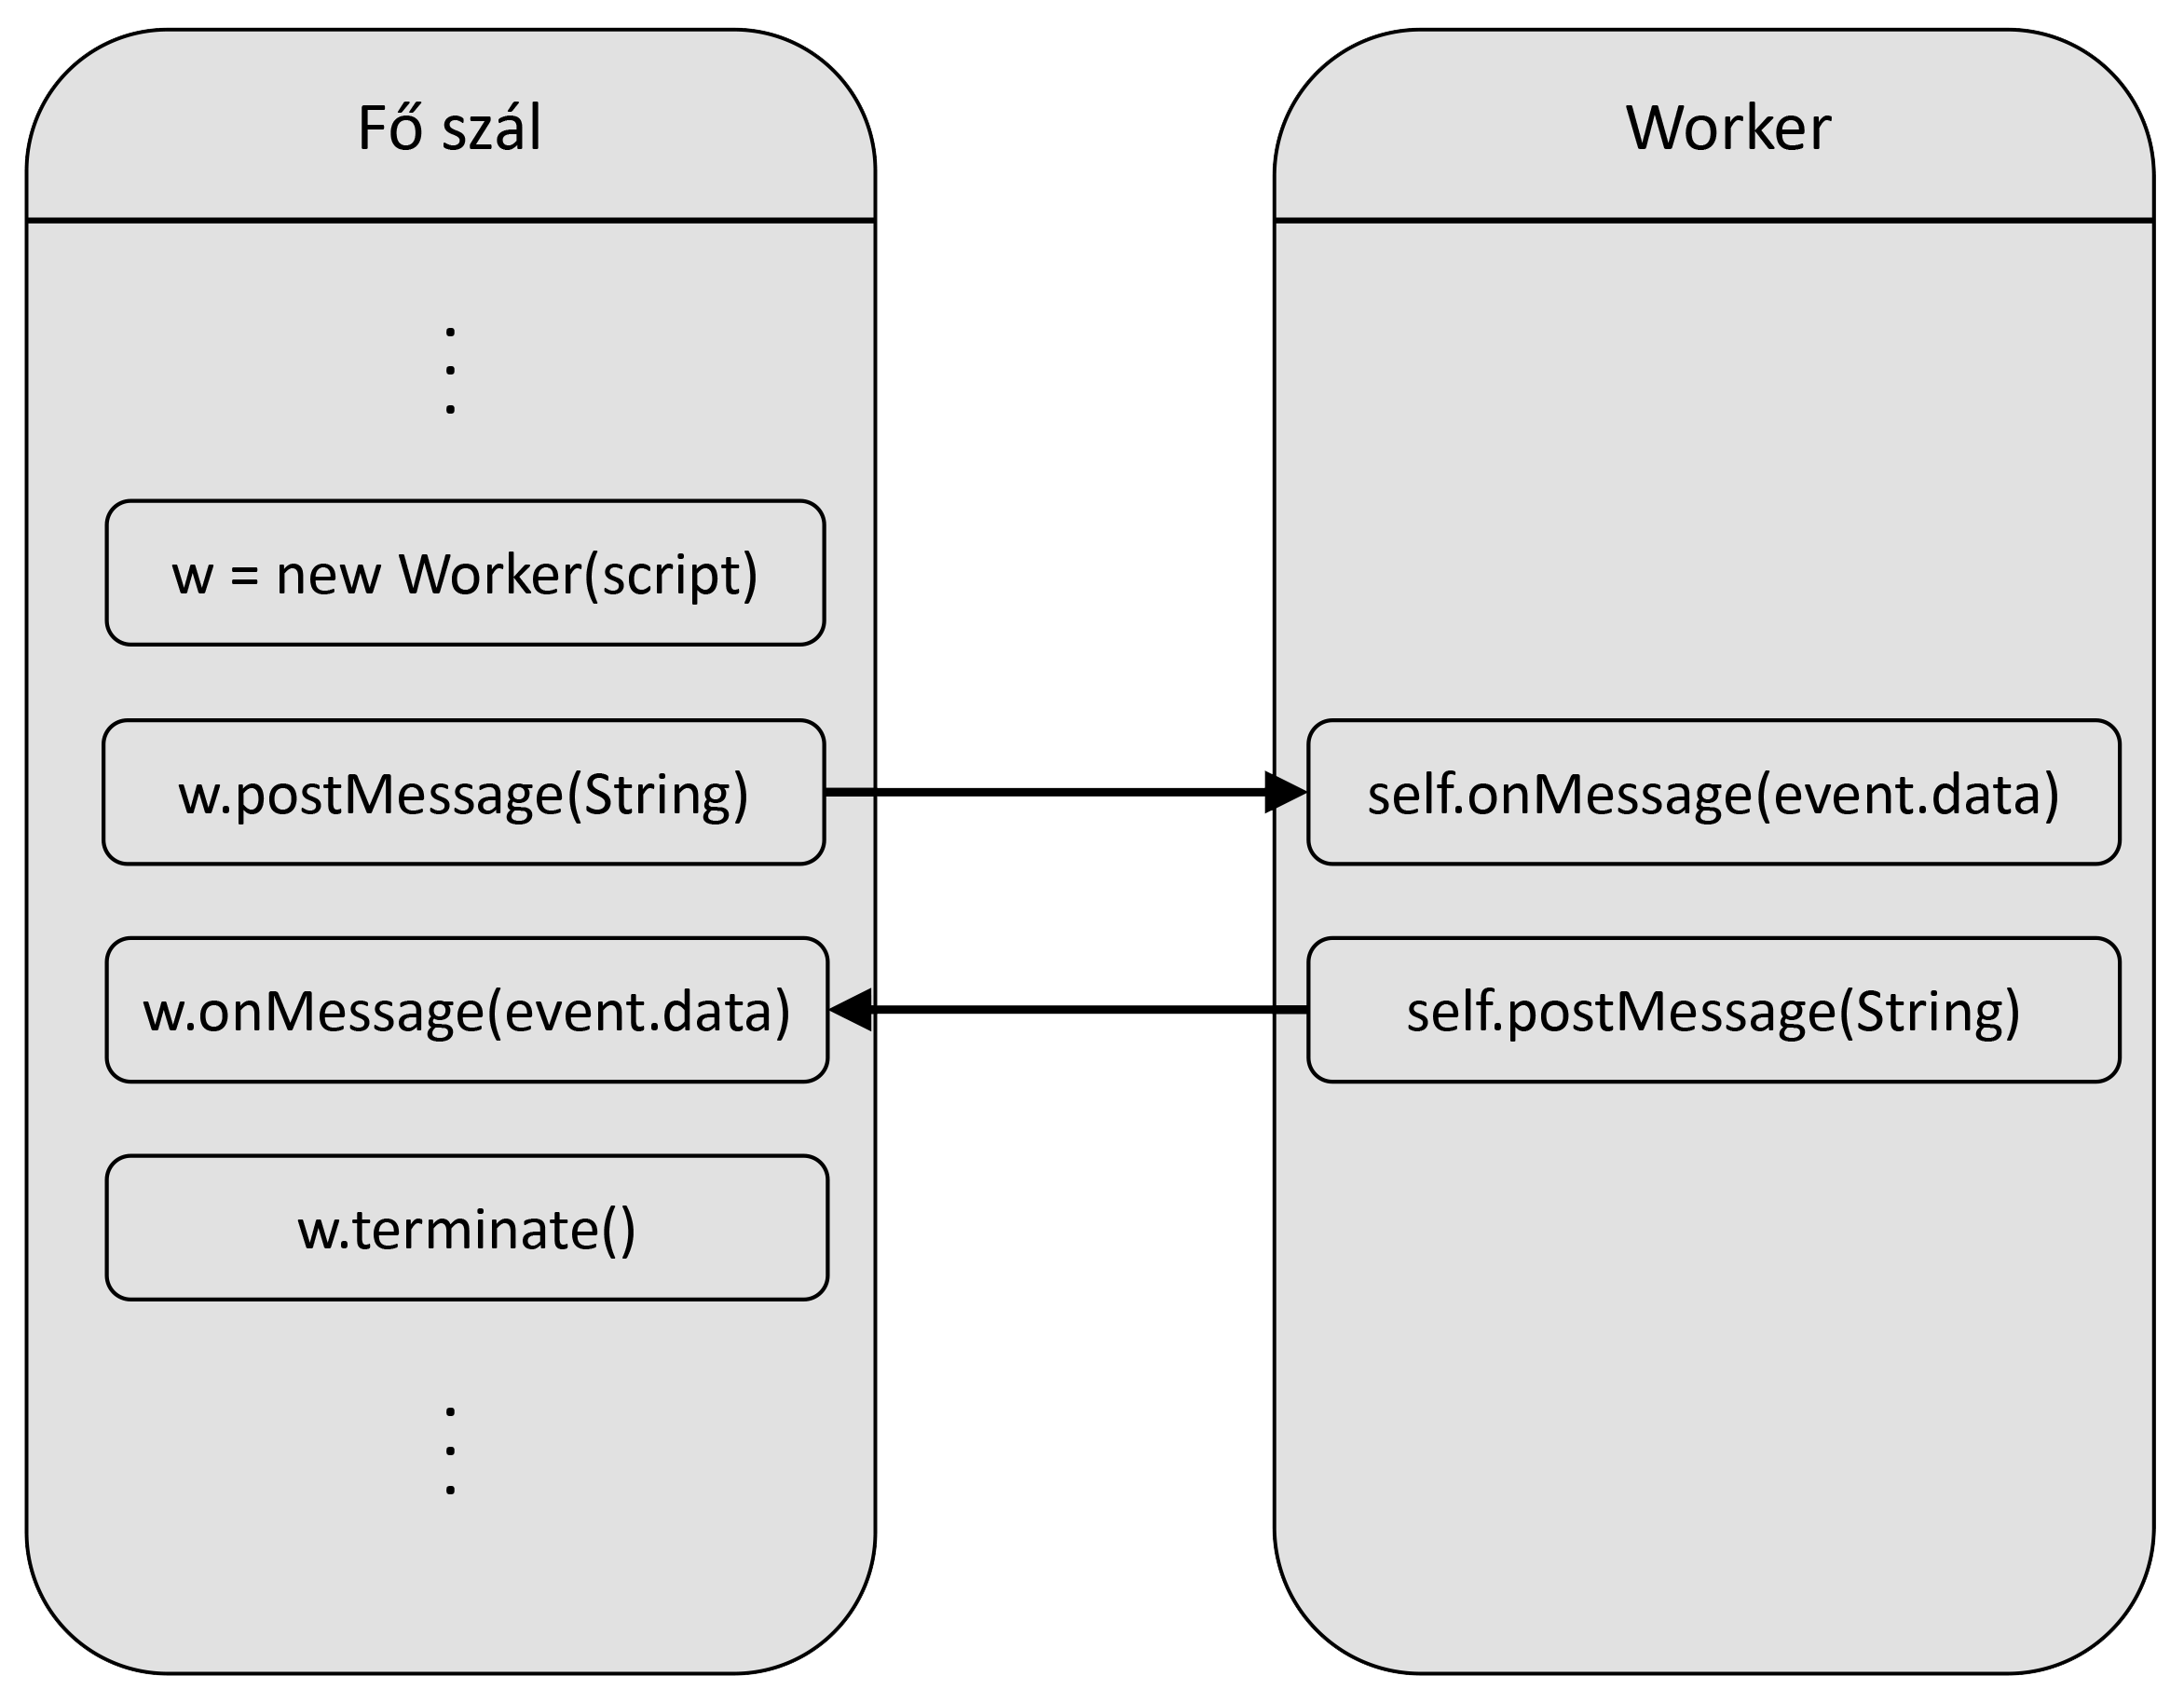
\includegraphics[scale=0.6]{images/Worker.png}
\caption{JavaScript Web Worker technológiájának működése.}
\label{fig:jsww}
\end{figure}

\begin{itemize}
\item A Worker konstruktornak meg kell adni az elérési útját annak a JavaScript fájlnak, amiben a párhuzamosítandó kód szerepel.
\item Az objektum postMessage függvényén keresztül lehetséges az üzenet küldése mindkét irányba.
\item Az onMessage esemény figyeli, hogy küldtek-e üzenetet vagy sem.
\item A terminate függvényhívással törölhetjük a workert a böngészőből.
\end{itemize}
\newpage
\Section{CSS}

A weboldal vázát, ha megszerkesztettük a HTML leíró nyelvvel, akkor az alapértelmezett stílusleírást fogja megkapni minden elem. Ahhoz, hogy a kreativitásunknak ne szabjanak határt, létrehozták a CSS stílusleíró nyelvet hat évvel a HTML megjelenése után. Ez egy olyan erőteljes eszközt ad a kezünkbe, amellyel bármilyen weboldal elkészíthető. A stílusok beállítására hivatkozni szükséges a módosítandó elemekre melynek egyszerűbb módjai:
\begin{enumerate}
  \item elem (tag) kiválasztás \begin{HTML5}
p {
    background-color: yellow;
}
\end{HTML5}
  \item egyedi azonosító (id) kiválasztás \begin{HTML5}
#title { ... }
\end{HTML5}
  \item csoport (class) kiválasztás \begin{HTML5}
.paragraphs { ... }
\end{HTML5}
\end{enumerate}
A stílusok megadásának három lehetséges megadási formája létezik, ezek érvényesülés sorrendjében a:
\begin{enumerate}
  \item Külső (external) stílus \begin{description}
  \item[] Egy külön .css fájlban definiáljuk az elemek tulajdonságait. A CSS fájlt a HTML \codeword{<head>} részében szükséges importálni, melynek módja: \begin{HTML5}
<link rel="stylesheet" href="style/style.css">
\end{HTML5}
\end{description}

  \item Belső (internal) stílus \begin{description}
  \item[] A HTML dokumentum \codeword{<head>} részében is létrehozhatunk egy \codeword{<style>} elemet, melyben ugyanúgy kell megadni a stílusokat, mint a külső változatánál. \begin{HTML5}
<style>
body{
    background-color: lightblue;
}
</style>
\end{HTML5}
\end{description}
  \item Sorközi (inline) stílus \begin{description}
  \item[] Közvetlenül az elemek style attribútumában is lehet rögzíteni a stílusokat. \begin{HTML5}
<h1 style="color: blue; text-align: center;">Ez egy cimsor</h1>
\end{HTML5}
\end{description}
\end{enumerate}

\newpage
\Section{Bootstrap 4}

Az internet fiatal korában többféle könyvtárat használtak interfészek készítéséhez, mely megnehezítette a karbantartását a weboldalaknak. Mark Otto, a Twitter egyik fejlesztője rukkolt elő azzal az ötlettel, hogy megalkot egy rendszert, mely kielégíti a kor követelményeit a webfejlesztés terén, így jelent meg 2011-ben a Bootstrap.

A Bootstrap egy ingyenes, nyílt forráskódú CSS keretrendszer, amely a front-end fejlesztést segíti azáltal, hogy támogatást nyújt reszponzív felületek létrehozásához. Elsősorban CSS alapú, de tartalmaz JavaScript-re épülő sablonokat is. Definiáltak például űrlapokat, gombokat, menürendszert és még sok mást. Ezeket a sablonokat úgy lehet alkalmazni, hogy a megfelelő class-szal ellátjuk az elemet. Például:
\begin{HTML5}
<button class="btn btn-primary btn-block"></button>
\end{HTML5}

A Bootstrap az elemek csoportokba rendezéséhez konténereket definiált több méretben. Hat lehetőség közül lehet választani, ezek között az a különbség, hogy milyen képernyőszélesség alatt töltik ki az oldalt teljes szélességében. Ezeket a konténereket feldarabolhatjuk több részre, és így egy rácsszerkezetet hozhatunk létre a weboldalon. Tizenkét darab oszlop hozható létre maximálisan, viszont ezt úgy töltik ki a benne foglalt mezők, ahogy szeretnénk. Egy mezőnek meg lehet adni, hogy hány egységet töltsön ki a tizenkét oszlopból. Ezt az értéket az összes konténer méretre lehet rögzíteni, melyet a következő példán szemléltetek.

\begin{figure}[ht]
\centering
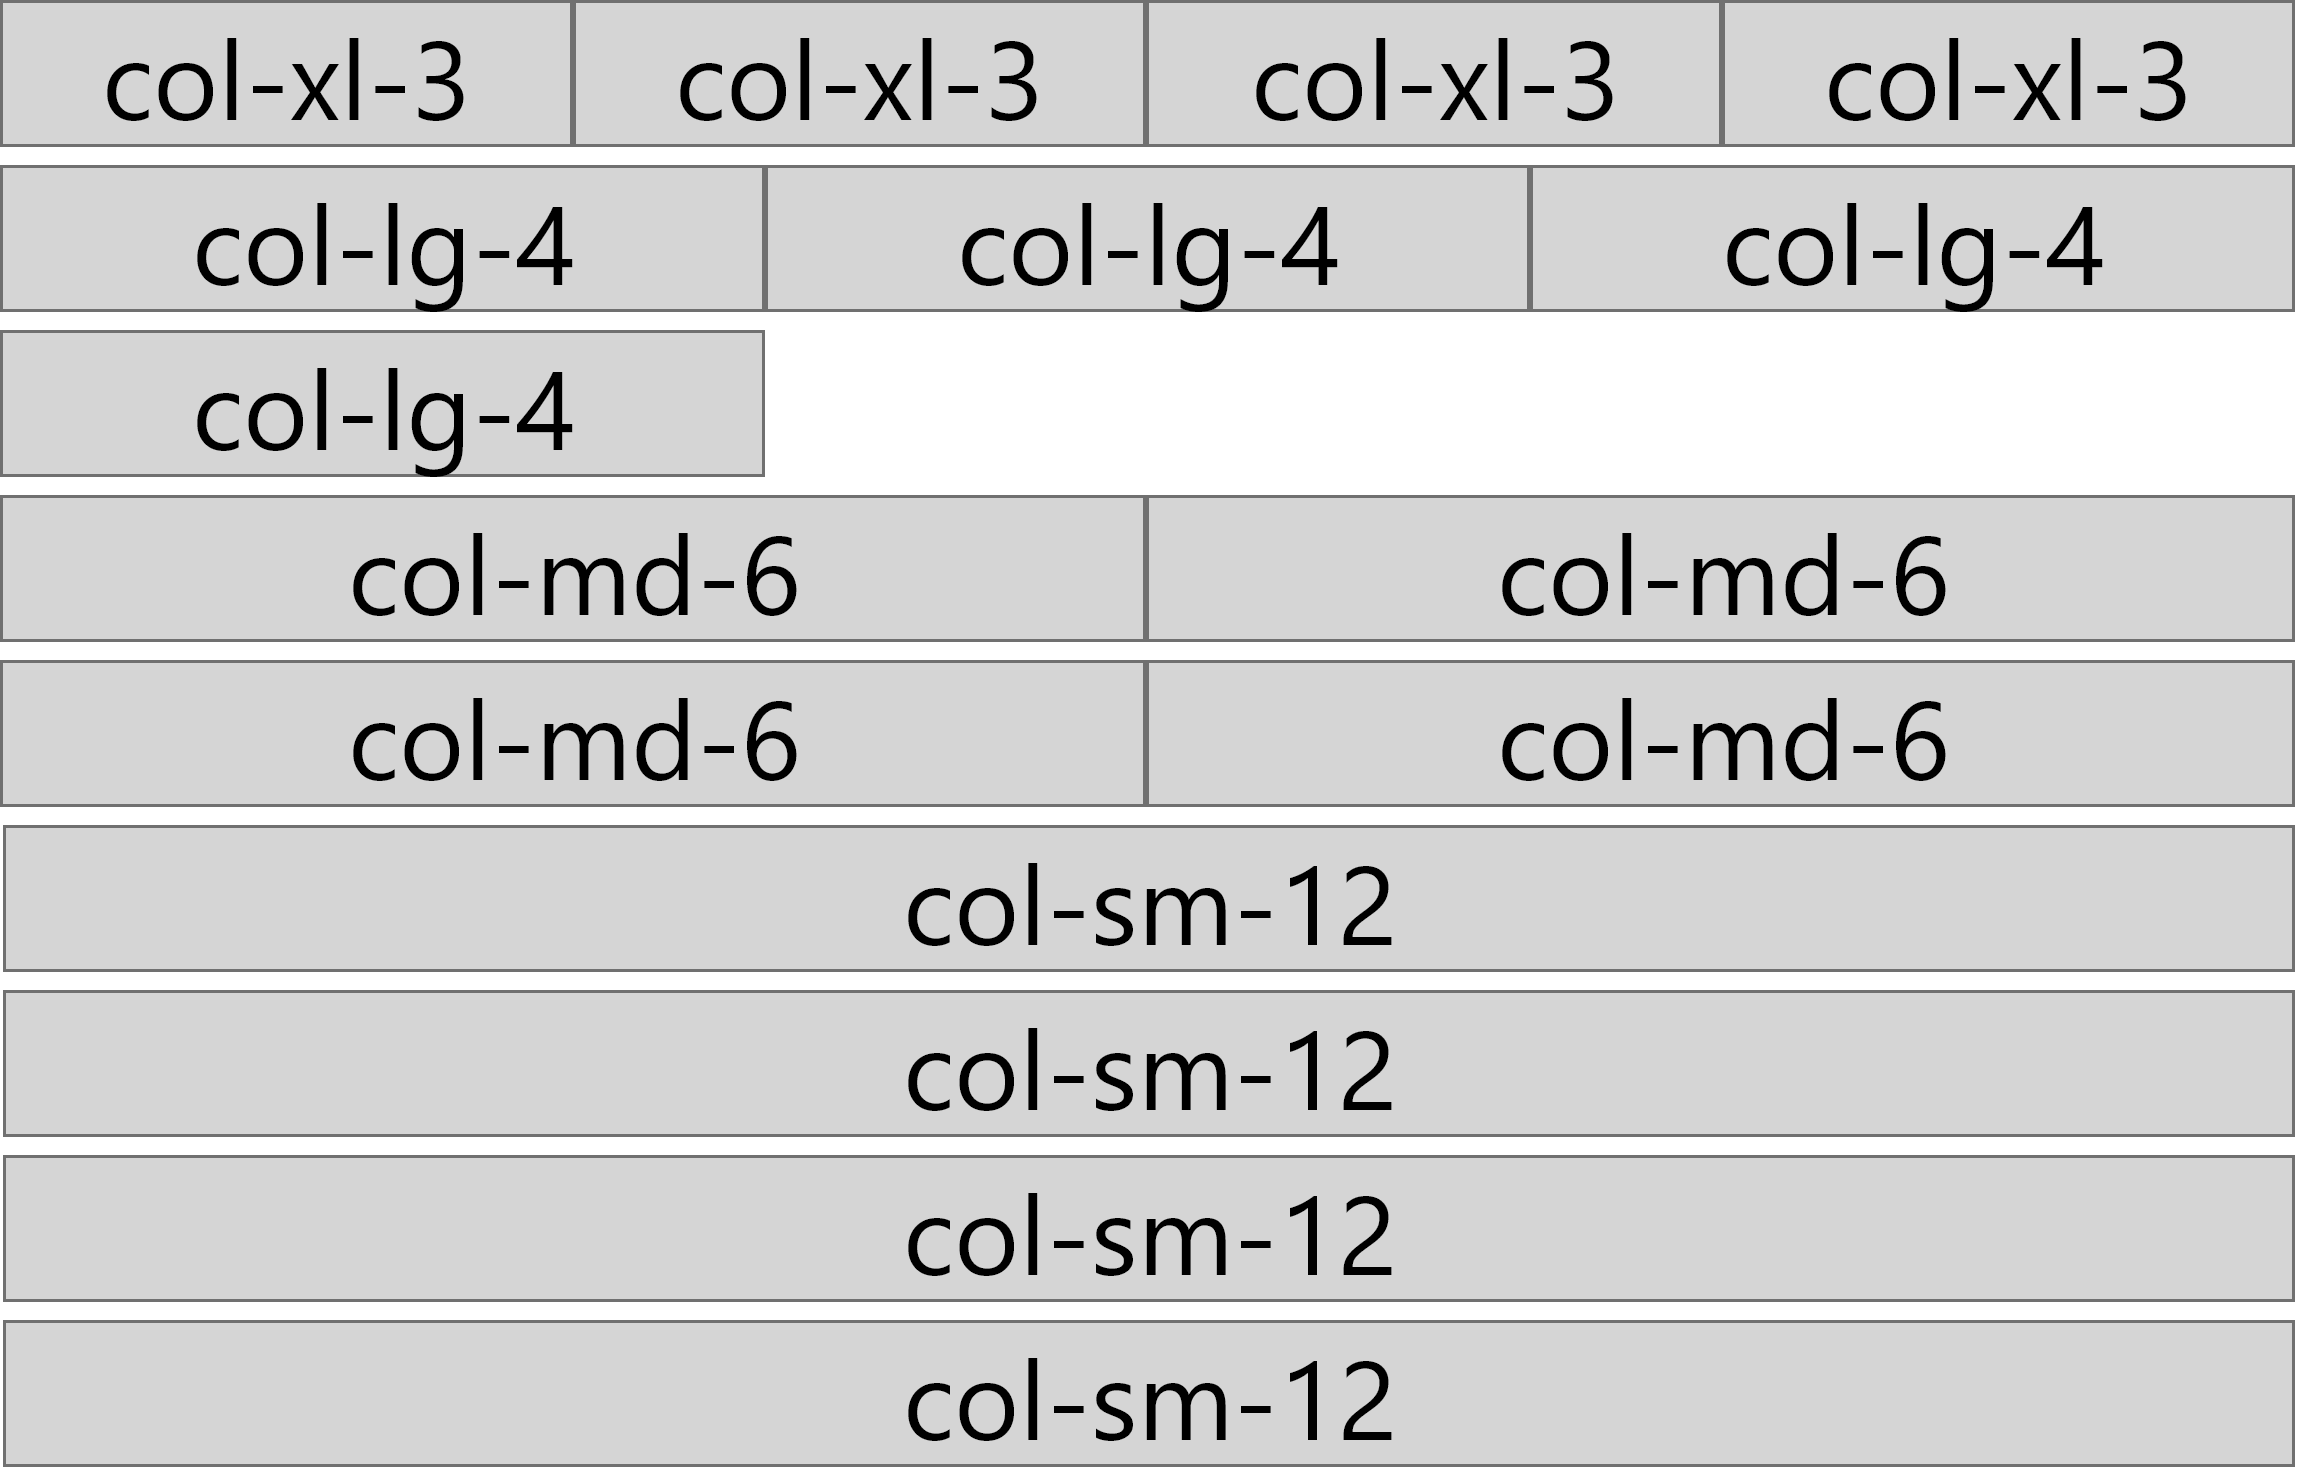
\includegraphics[scale=0.15]{images/bootstrap.png}
\caption{Bootstrap 4 rácsszerkezete.}
\label{fig:bs4}
\end{figure}
\noindent Ha teljes méretben tekintjük meg a weboldalt, akkor egymás mellett elférnek a mezők, viszont minél inkább csökken a weboldal szélessége, annál több helyet vesz fel egy-egy mező, s elkezdi új sorba rendezni a fennmaradókat. A mezők azt a class értéket tartalmazzák \aref{fig:bs4} ábrán, amivel beállíthatóak ezek az méretek \cite{Bootstrap}.

\newpage

\Section{Genetikus algoritmus}
A számítástechnikában a genetikus algoritmusok optimalizációs eljárások, melyek a biológia evolúciós elvekeit követik, mint a mutáció, keresztezés, és a kiválasztás. Abban az esetben megfelelő választás, amikor az optimum egy közelítése is elegendő a megoldáshoz, mert sok esetben előfordulhat, hogy nagyon sok munka lenne előállítani a tökéletes megoldást. A genetikus algoritmus építőelemei a kromoszómák, a fitness alapú kiválasztás és a biológiából átvett műveletek. A kromoszóma tipikusan egy bináris string formátumot vesz fel. A kromoszómákon belül minden egyes lokusznál (ahol a gén található) kettő lehetséges allél létezik: 0 és 1.
\begin{figure}[ht]
\centering
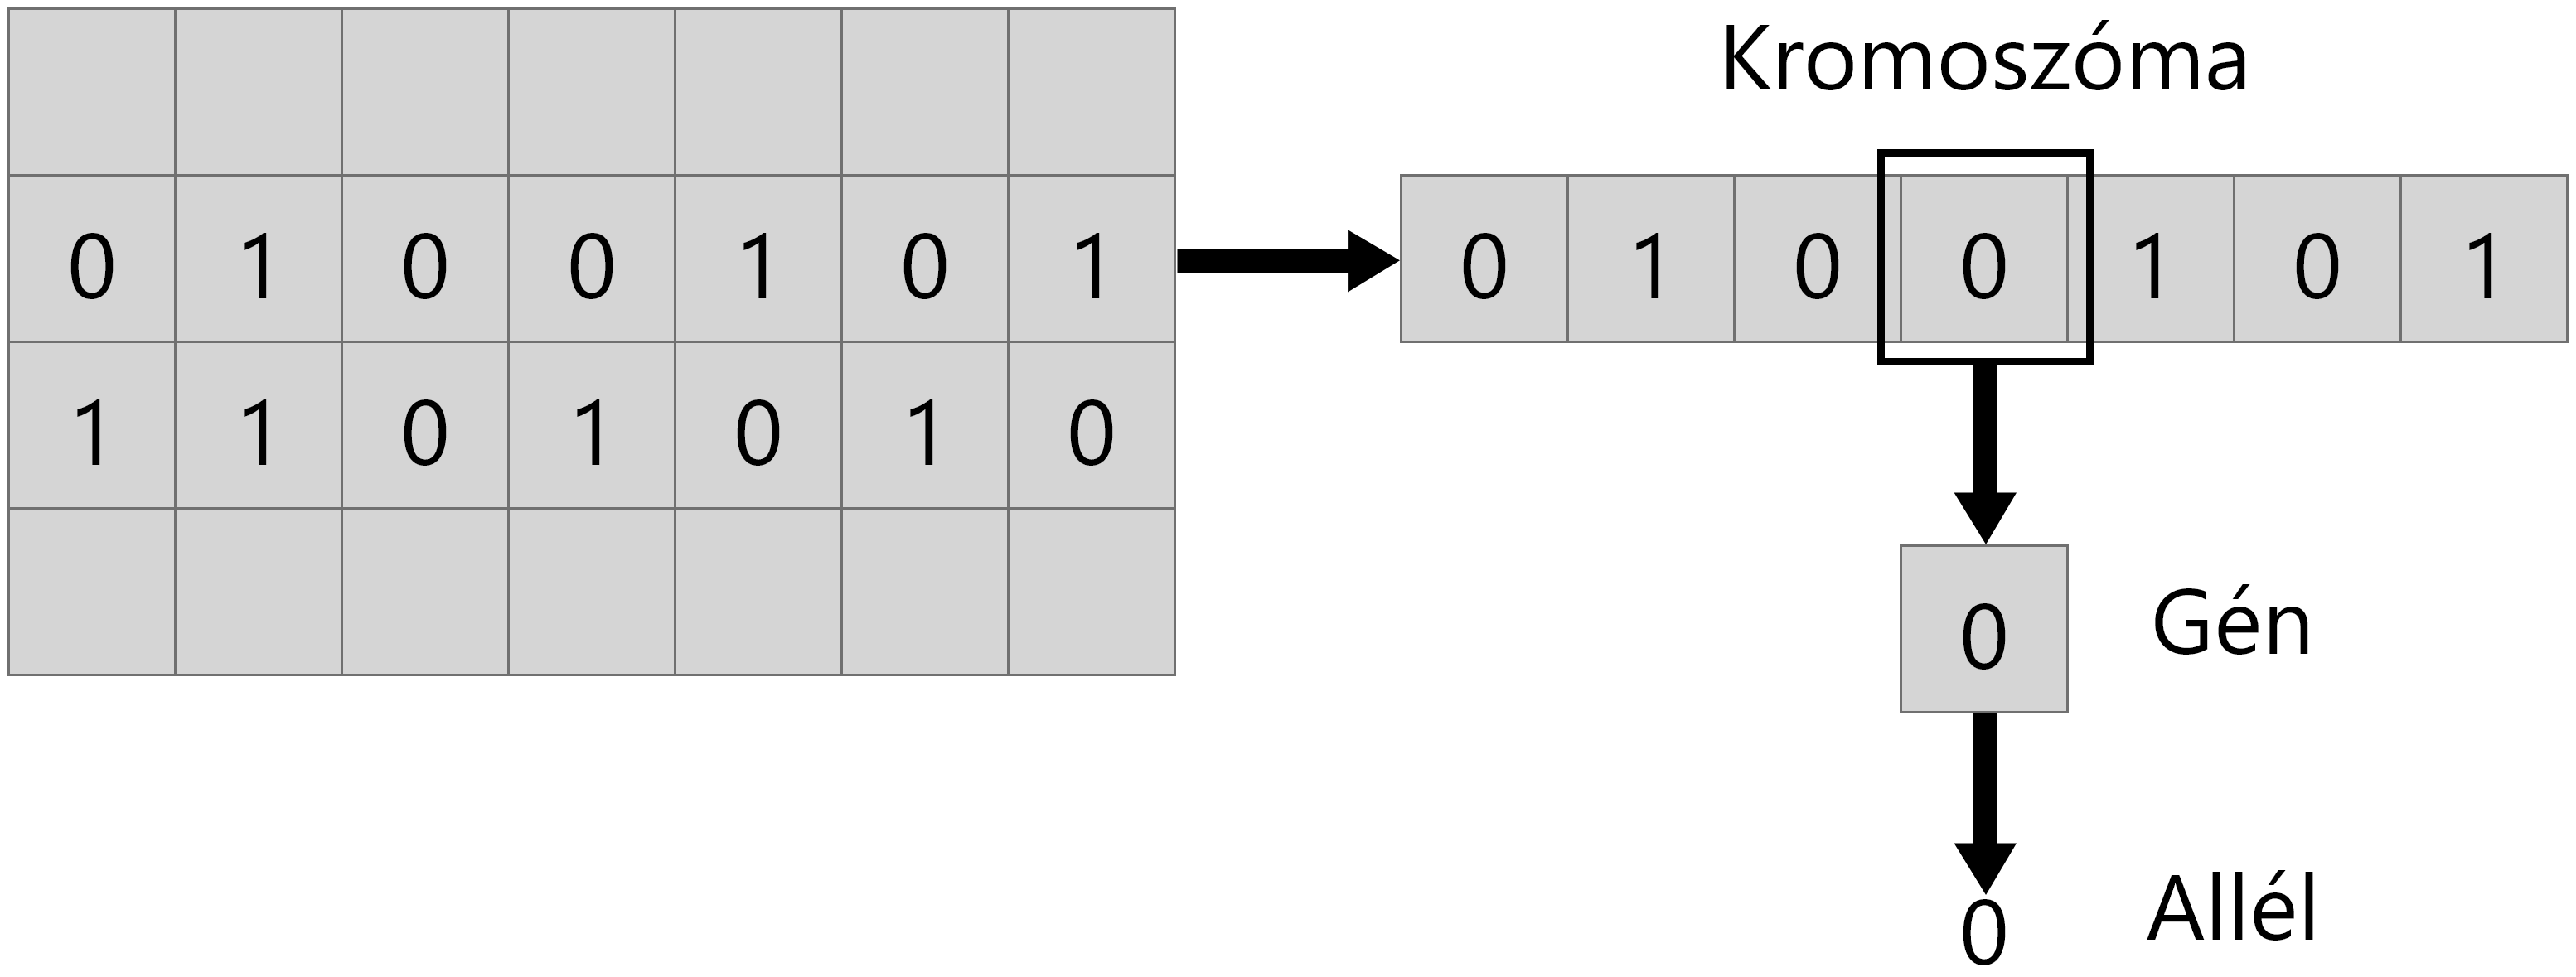
\includegraphics[scale=0.13]{images/kromoszoma.png}
\caption{Populáció felépítése.}
\label{fig:kromo}
\end{figure}

\noindent A kromoszóma tulajdonképpen a megoldás halmaz egy pontja. Ezeket a kromoszómákat dolgozzuk fel a genetikus operátorokkal. Azt, hogy mennyire elfogadható a megoldás, az $f(x) \to \mathbb{R}$ fitness függvény mutatja meg, mely a valós számok halmazába képez le. A biológiai operátorok közé tartozik a kiválasztás, a mutáció és a keresztezés. A kiválasztásnál a fitness függvény alapján választunk ki kromoszómákat. A keresztezés operátor két kromoszóma esetén egy-egy véletlen lokuszt választ ki, mely mentén két részre osztódnak a kromoszómák, s az utolsó szeletüket felcseréljük. Mutációkor a kromoszóma egy-egy génjében felcserélődik az allél.
\begin{figure}[ht]
\centering
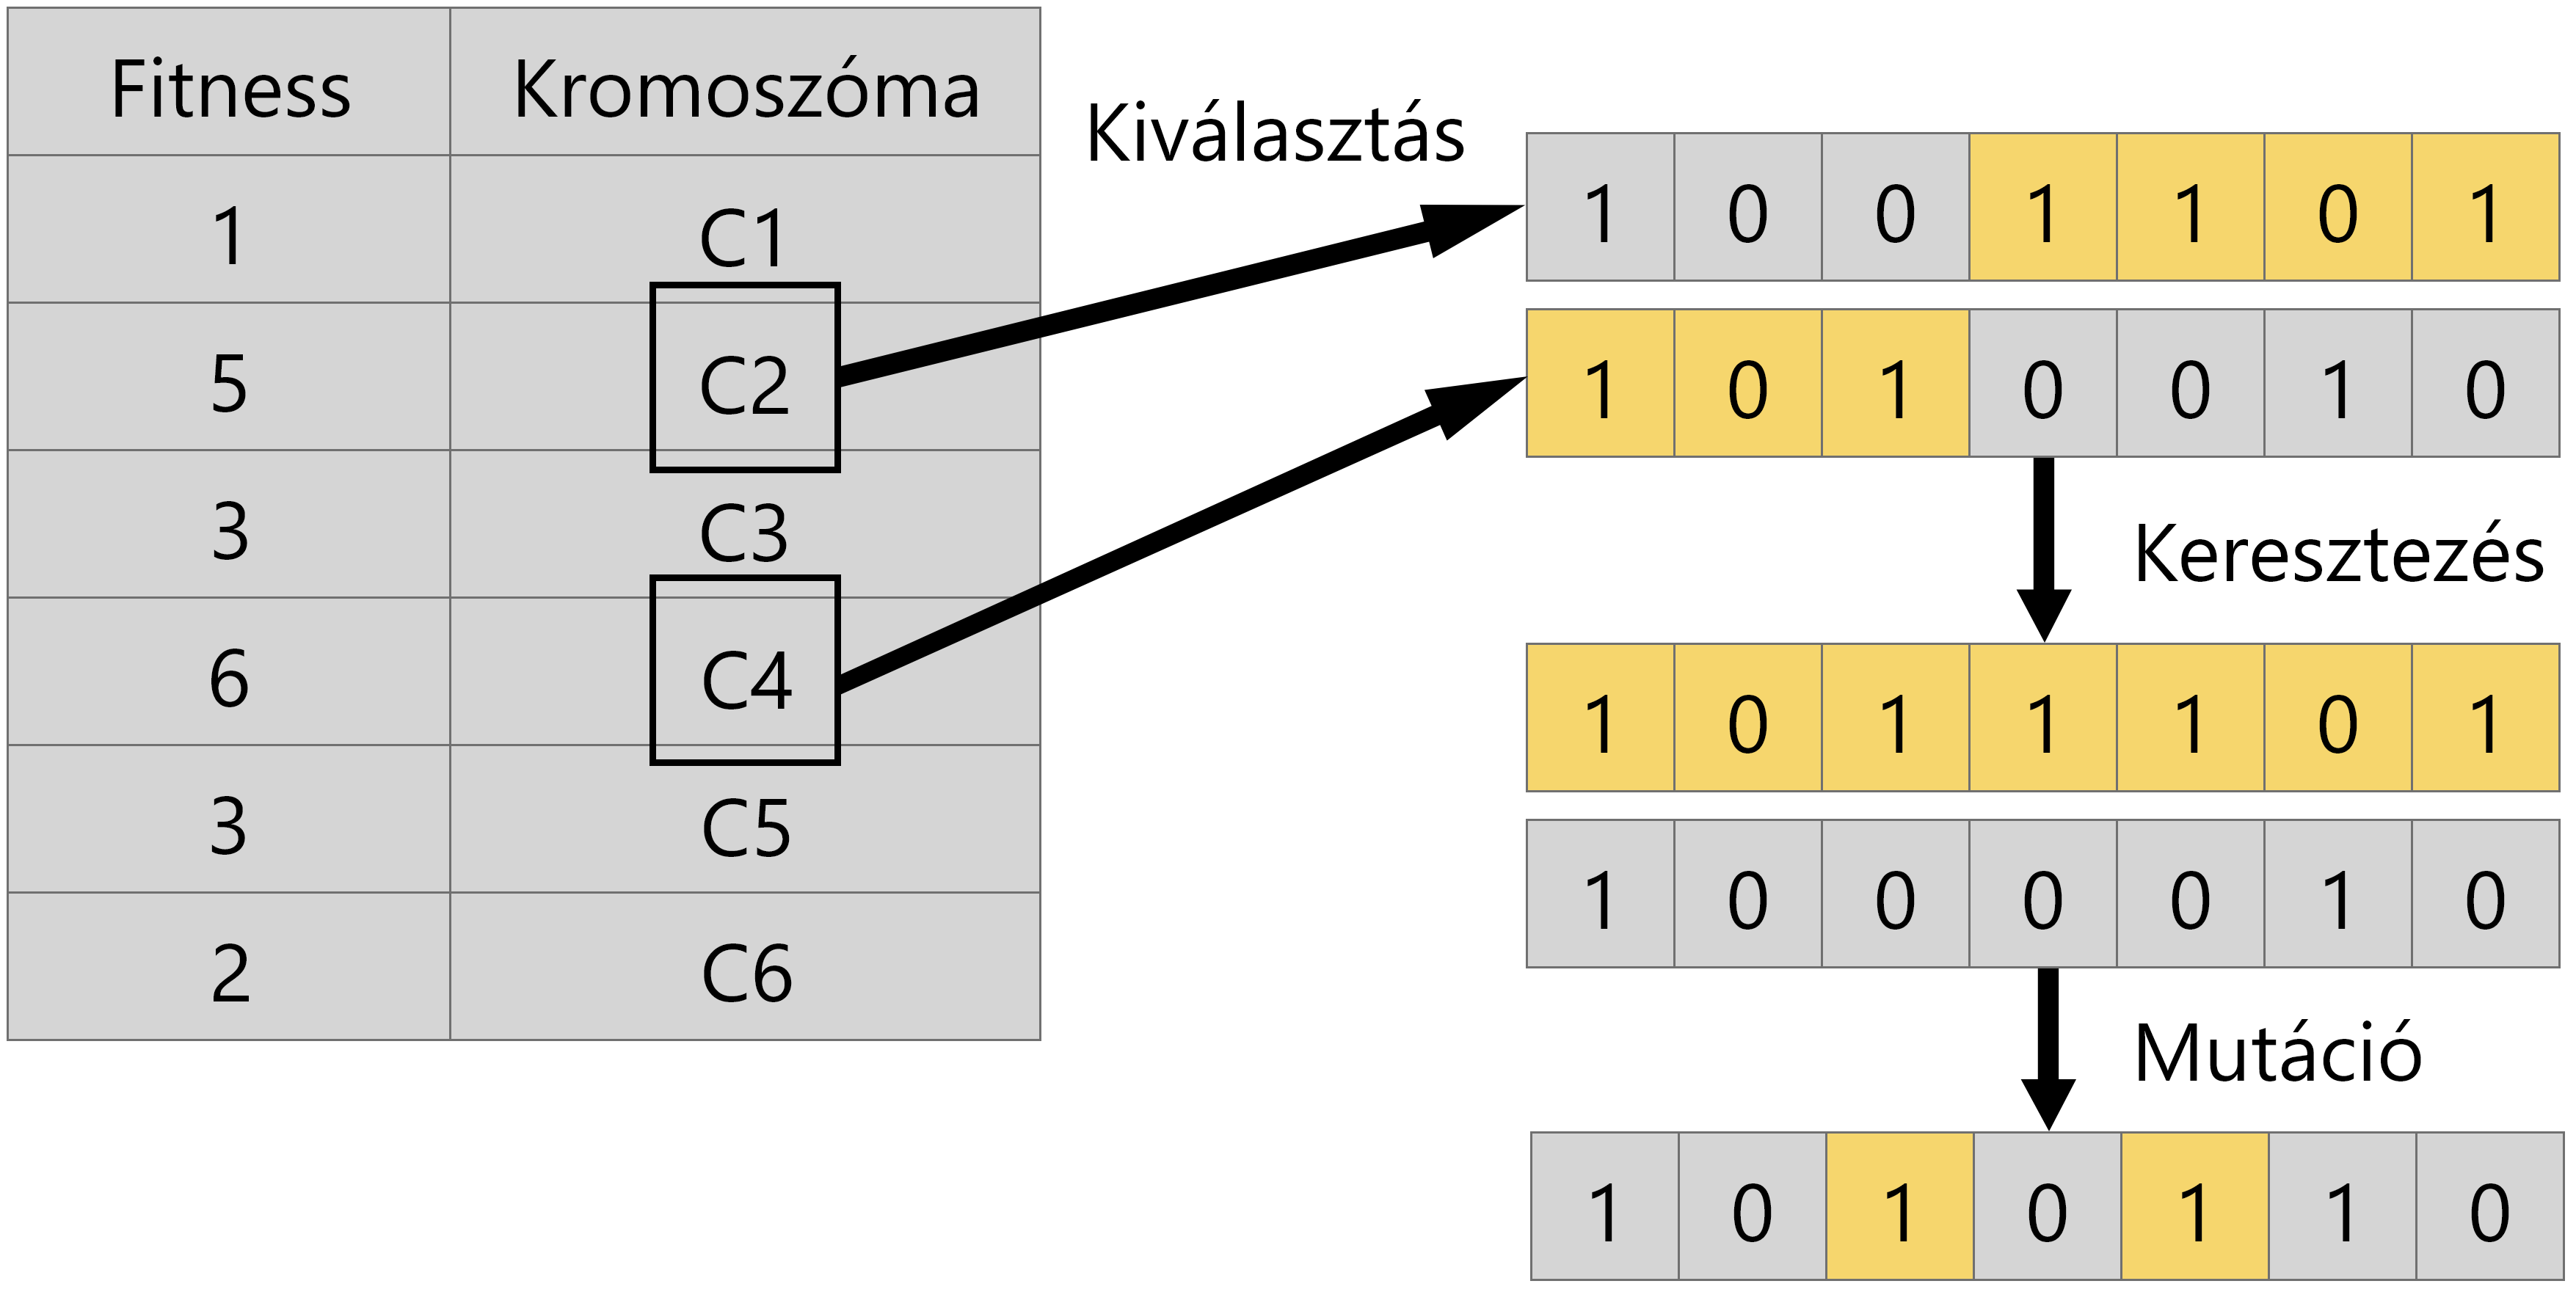
\includegraphics[scale=0.11]{images/mutacio.png}
\caption{Kromoszómákon végzett műveletek.}
\label{fig:mutac}
\end{figure}

\newpage

\Section{Alpha Vantage}
\label{alphavantage}
Az Alpha Vantage egy adatszolgáltató cég, weboldal. Több nagyobb vállalattal partnerséget kötve jött létre ez az adattár, mely ingyenesen biztosít kutatási és egyéb célra napi, havi, vagy akár napközben rögzített részvény adatokat. Nemcsak cégek tőzsdei értékeivel foglalkoznak, hanem kriptovalutákra is található itt adat, amellyel kiegészülve széles spektrumúnak tekinthető a szolgáltatás. A használatához szükség van egy API key-re, mely azonosítja a felhasználót a lekérdezések során. Az ingyenes kulcs mellett korlátozásokat fogalmazott meg a cég, napi 500, illetve percenként 5 a maximum hívások száma, ami megengedett. Ez kibővíthető, vannak prémium opciók, viszont ez az adatokra semmilyen pozitív hatással nincsen.

Az Alpha Vantage API több lehetőséget is kínál, részletesen a napi kereskedéshez kapcsolódó információkat mutatom be. A \textbf{TIME\_SERIES\_INTRADAY} lekérdezés során lehetőség van 1-2 hónap adatait kinyerni, amely gyorsabb letöltést tesz lehetővé, illetve, ha csak kisebb mennyiségű adatra van szükség, akkor ezt célszerű használni. A lekérdezéshez több kapcsoló tartozik, melyeket részletezek a következő sorokban, vastagon szedve a kötelező paramétereket.

\begin{itemize}
  \item \textbf{function}: itt adható meg, hogy melyik lekérdezési formát szeretnénk használni, ez esetben TIME\_SERIES\_INTRADAY.
  \item \textbf{symbol}: ez a kapcsoló adja meg a tickert, a részvény azonosítóját, például: GOOG, AAPL, TSLA.
  \item \textbf{interval}: két egymást követő adat között eltelt időt határozza meg, ez lehet 1, 5, 15, 30 és 60 perces.
  \item adjusted: ez a kapcsoló határozza meg, hogy korrigált legyen-e a részvény értéke vagy sem. Alapértelmezésképp ez igaz, hiszen, ha a részvényt például kettéosztják (split), az értéke hirtelen a felére csökken, s ha nem vagyunk tudatában annak, hogy ez történt, akkor tévesen hihetjük azt, hogy csökkent az érték, el kell adni a papírokat.
  \item outputsize: lehet compact, vagy full. A compact az alapértelmezett érték, így csak 100 értéket kapunk vissza az oldaltól. Ha a full kapcsolót használjuk, akkor a teljes méretű adatsort kapjuk vissza.
  \item datatype: kettő visszatérési forma közül lehet választani, a JSON és a CSV. A JSON elterjedt a webes alkalmazások körében, ezért ez az alapértelmezett, viszont ezzel szemben a CSV egyszerű, s kompatibilis a széles körben használt Excel programmal.
  \item \textbf{apikey}: a kapott kulcsot itt kell megadni.
\end{itemize}

Az én felhasználásomhoz egy bővebb adathalmazra van szükség, melyre egy másik függvény, paraméter meghívása szükséges a weboldalon, a \textbf{TIME\_SERIES\_IN\-TRADAY\_EXTENDED}. Ez a függvény visszatér két évre visszamenőleg az adatokkal, amelyet ők is ajánlanak szimulációkhoz, vizualizációhoz. Az előző függvénytől nem tér el sokban, kikerült a datatype kapcsoló, hiszen a CSV kevésbé memóriaigényes mint a JSON, s a helyére a slice kapcsoló került be, mellyel a különböző darabjait tudjuk letölteni az adatsornak. A két év minden hónapját külön tudjuk lekérdezni, példa a használatra: slice=year1month1. Ennek a függvénynek a visszatérési fájlja a következő adatokat tartalmazza:
\begin{itemize}
  \item Date: az részvény árának mintavételi dátuma,
  \item Open: a nyitóár,
  \item High: a maximum érték,
  \item Low: a minimum érték,
  \item Close: a záróár,
  \item Volume: a részvények mennyisége.
\end{itemize}

Egy példa lekérdezés az alábbiak szerint hívható meg.

\noindent
\newsavebox\lstA
\begin{lrbox}{\lstA}
\begin{HTML5}
https://www.alphavantage.co/query?
function=TIME_SERIES_INTRADAY_EXTENDED&symbol=IBM
&interval=15min&slice=year1month1&apikey=demo
\end{HTML5}
\end{lrbox}
\href{https://www.alphavantage.co/query?function=TIME_SERIES_INTRADAY_EXTENDED&symbol=IBM&interval=15min&slice=year1month1&apikey=demo}{\usebox{\lstA}}



\noindent Paramétereit tekintve elmondható, hogy az IBM vállalat részvényeit adja vissza az elmúlt 30 napból, 15 perces időközökkel \cite{AlphaVantage}.

\Section{Highcharts}
A szimulációk egyik fontos eleme a megfelelő grafikai szemléltetés. Sokkal érthetőbb lesz az eredmény, hogyha valamilyen ábrát, táblázatot, grafikont jelenítünk meg. Az elemzéseim megjelenítéséhez a Highcharts termékét választottam, a Stock-ot. Ez egy alapvetően fizetős fejlesztői könyvtár, azonban egyetemistáknak ingyenesen is rendelkezésre bocsátják, csupán egy egyszerű űrlapot kell kitölteni és máris küldik emailben a letöltési linket. A weboldalon rengeteg demo programot lehet megtekinteni, szinte mindenre található valamilyen példa. A táblázat megadása objektum formában történik meghatározott paraméterek alapján. Például egy egyszerű vonaldiagram megadható a következő módon.
\begin{javascript}
Highcharts.chart('container', {
    title: {
        text: 'Title'
    },
    series: [{
        data: [1, 2, 4, 8, 16, 32, 64, 128, 256],
        pointStart: 1
    }]
});
\end{javascript}
A függvényhívás első paramétere lesz az a \codeword{<div>} ahova fogja kirajzolni a grafikont, a következő paraméter pedig egy objektum, amiben különféle paramétereket adhatunk meg. Jelen esetben két paraméter szerepel benne, a title, vagyis a címe a grafikonnak, illetve a series, amiben az adatokat szükséges megadni. Ha szeretnénk egy újabb vonalat ugyanerre az ábrára rajzolni, akkor a series tömbhöz egy újabb objektumot szükséges hozzáadni \cite{Highcharts}.
\begin{figure}[ht]
\centering
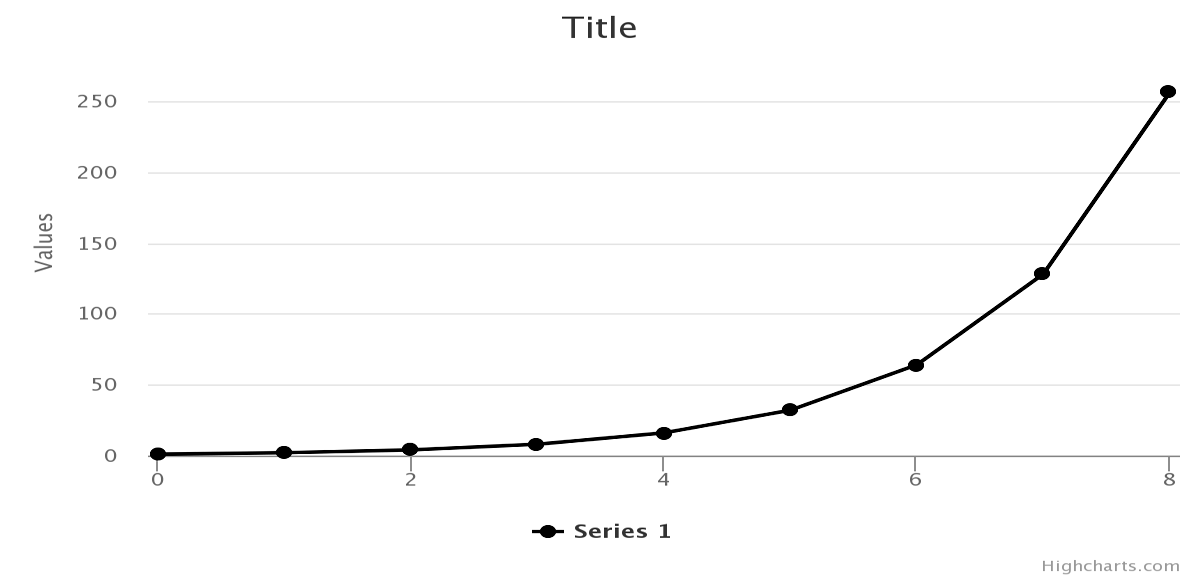
\includegraphics[scale=0.35]{images/highchart.png}
\caption{Vonaldiagram a Highchart környezetben.}
\label{fig:highchart}
\end{figure}

Amennyiben részvényspecifikus ábrákat szeretnénk megjeleníteni, arra is lehetőséget ad a Highcharts. Kis módosítással létrehozhatunk egy gyertyadiagramot, ahol egyszerre több adatot is megtudhatunk a részvény áráról.
\begin{figure}[ht]
\centering
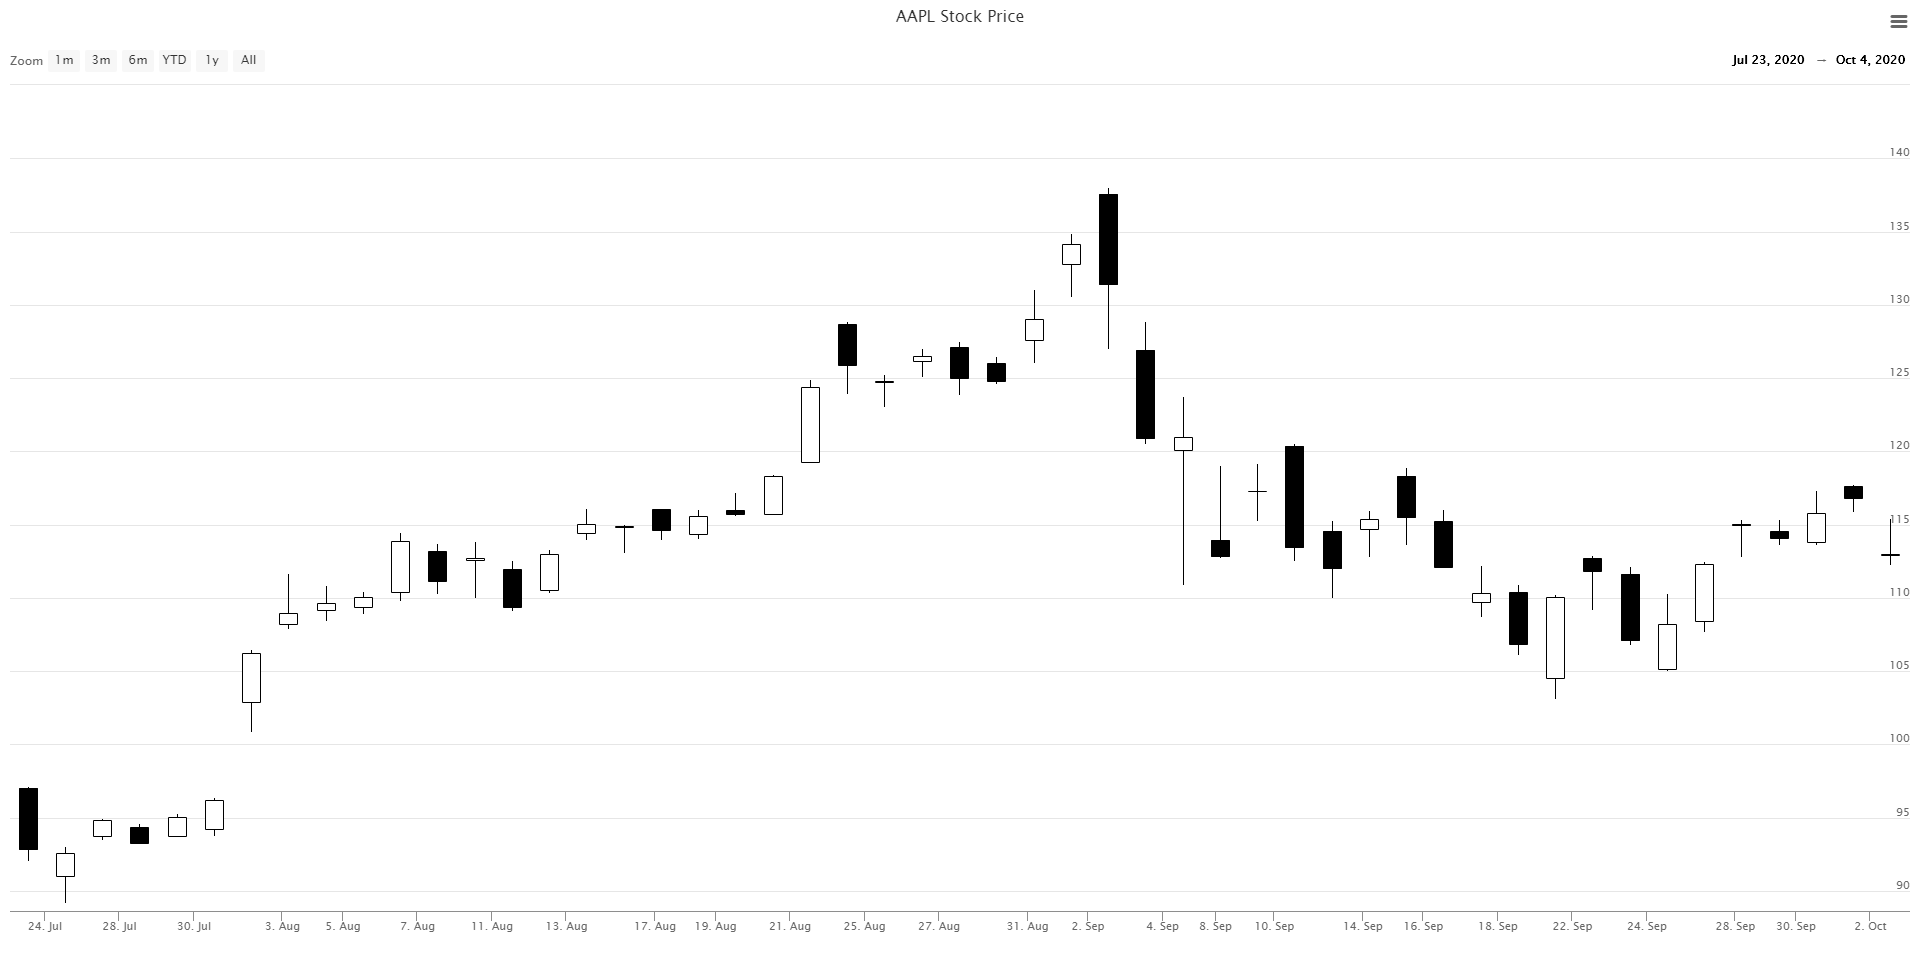
\includegraphics[scale=0.22]{images/highchart_stock.png}
\caption{Gyertyadiagram a Highchart környezetben.}
\label{fig:highchart_stock}
\end{figure}

\begin{javascript}
Highcharts.stockChart('container', {
    title: {
      text: 'AAPL'
    },series: [{
      type: 'candlestick',
      name: 'AAPL',
      data: data}]
});
\end{javascript} 